\documentclass[fleqn, a4paper, 11pt, russian]{article}

\usepackage[utf8]{inputenc}
\usepackage[T1, T2A]{fontenc}
\usepackage[english, main = russian]{babel}
\usepackage{pscyr}
\usepackage{indentfirst}
\parindent 1.27cm
\usepackage{graphicx}
\usepackage{natbib}
\usepackage{caption, subcaption}
\usepackage[top=2cm, left=2cm, right=2cm, left=2cm]{geometry}
\usepackage{amsmath} %Для работы с матрицами
\usepackage{ragged2e}
\usepackage{adjustbox}
\usepackage{makecell}
\usepackage{multirow}

\graphicspath{{Graphics/Images/}}

\captionsetup[figure]{name = Рисунок, labelsep = endash}
\captionsetup[table]{name = Таблица, labelsep = endash, justification=raggedright, singlelinecheck=false}
\setlength{\mathindent}{0pt}

\begin{document}
	\newcommand\tline[2]{$\underset{\text{#1}}{\text{\underline{\hspace{#2}}}}$}

\begin{titlepage}
	\centering
	{\fontsize{12pt}{5cm}\selectfont \bfseries Министерство образования и науки Российской Федерации} \\ \vspace{0.5cm}
	{\fontsize{7pt}{5cm}\selectfont ФЕДЕРАЛЬНОЕ ГОСУДАРСТВЕННОЕ АВТОНОМНОЕ ОБРАЗОВАТЕЛЬНОЕ УЧРЕЖДЕНИЕ ВЫСШЕГО ПРОФЕССИОНАЛЬНОГО ОБРАЗОВАНИЯ} \\ 
	\vspace{1cm}
	{\fontsize{12pt}{5cm}\selectfont \bfseries САНКТ-ПЕТЕРБУРГСКИЙ УНИВЕРСИТЕТ ИНФОРМАЦИОННЫХ ТЕХНОЛОГИЙ, МЕХАНИКИ И ОПТИКИ} \\ \vspace{1.5cm}

	{\fontsize{14pt}{5cm}\selectfont Кафедра \hspace{1cm} \underline{Систем Управления и Информатики}  \hspace{1cm} Группа \underline{Р3340}} \\ 
	\vspace{2cm}

	{\fontsize{20pt}{5cm}\selectfont \bfseries Лабораторная работа №7} \\
	{\fontsize{20pt}{5cm}\selectfont \bfseries “Анализ точности систем управления”} \\
	{\fontsize{14pt}{5cm}\selectfont Вариант - 2} \\
	\vspace{1.5cm}

	\flushleft

	{Выполнил \hspace{2cm} \underline{Алякин С.П.}\tline{(фамилия, и.о.)}{6.5cm} (подпись)} \\
	\vspace{2cm}

	{Проверил \hspace{2cm} \tline{(фамилия, и.о.)}{9cm} (подпись)} \\
	\vspace{5cm}

	"\underline{\hspace{0.7cm}}"\hspace{0.2cm}\underline{\hspace{2cm}}\hspace{0.2cm}20\underline{ 17 }г. \hspace{2cm} Санкт-Петербург, \hspace{2cm} 20\underline{ 17 }г. \\ \vspace{1cm}

	Работа выполнена с оценкой \hspace{1cm} \underline{\hspace{8cm}} \\ 
	\vspace{1cm}
	Дата защиты "\underline{\hspace{0.7cm}}"\hspace{0.2cm}\underline{\hspace{2cm}}\hspace{0.2cm}20\underline{ 17 }г.
		
\end{titlepage}
	\section*{Цель работы}
	Целью работы является изучение математических моделей и исследование характеристик исполнительного устройства, построенного на основе пьезоэлектрического двигателя микроперемещений.
	
	\section*{Исходные данные}
	Типовые конструкции пьезоэлектрических двигателей приведены на рисунке \ref{PEconstr}.
	\begin{figure}[ht!]
		\centering
		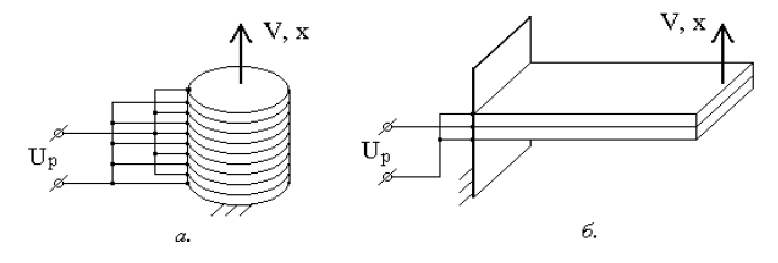
\includegraphics[width = 0.9\textwidth]{constructTypes}	
		\caption{Составная и биморфная конструкции пьезоэлектрических двигателей}
		\label{PEconstr}
	\end{figure}
	
	Исходные данные выполнения работы приведены в таблице \ref{initTab}.
	\begin{table}[h]
		\caption{Исходные данные}
		\begin{tabular}{|c|c|c|c|c|c|}
			\hline
			\makecell{$C_p,$\\Н/м} & \makecell{$m,$\\кг} & \makecell{$K_O,$\\Н/В} & \makecell{$K_d,$\\Н$\cdot$с/м} & \makecell{$T_u,$\\мс} & \makecell{$F_B,$\\Н}\\
			\hline
			$0,5\cdot10^8$ & 0,3 & 8,2 & $0,9\cdot10^3$ & $0,06$ & 80\\
			\hline	
		\end{tabular}
		\label{initTab}
	\end{table}
	
	В соответствии со вторым вариантом исследуется составной пьезоэлектрический двигатель, представленный на изображении \textit{а} рисунка \ref{PEconstr}.
	\clearpage
	\section{Составление передаточной функции двигателя}
	Для составления передаточной функции двигателя будем рассматривать пьезоэлектрическое устройство как упругую механическую систему. Тогда математическая модель может быть получена на основе уравнения баланса сил в пьезодвигателе:
	\begin{align}
		&&F_y = F_O + F_\text{Д} + F_d + F_B,
		\label{Feq}
	\end{align}
	где $F_y = C_p\cdot x, F_O = K_OU_p, F_\text{Д} = -m\displaystyle{\frac{d^2x}{d t}}$. Подставив перечисленные равенства в уравнение (\ref{Feq}), получим:
	\begin{align}
		&&m\ddot{x} + K_d\dot{x} + C_px = K_OU_p + F_B
	\end{align}
	
	Из этого при нулевом внешнем воздействии имеем передаточную функцию для пьезоэлектрического двигателя
	\begin{align} \label{Wpz}
		&&W_\text{ИУ}(s) = \displaystyle{\frac{K_O}{ms^2 + K_ds + C_p}}.
	\end{align}
	
	Управление ПД осуществляется с вольтного усилителя, который, в нашем случае, описывается апериодическим звеном первого порядка:
	\begin{align}
		&&W_\text{ВУ}(s) = \frac{K_u}{T_us + 1},
	\end{align}
	где $K_u = \displaystyle{\frac{U_{pm}}{U_m}} = \frac{300}{10} = 30.$
	
	Исходя из того, что ВУ и ПД соединены последовательно, имеем передаточную следующую функцию:
	\begin{align}
		&&W(s) = \frac{K_0\cdot K_u}{(T_us + 1)(ms^2 + K_ds + C_p)}.
	\end{align}
	\clearpage
	\section{Математическое моделирование пьезоэлектрического двигателя}
	Структурная схема пьезоэлектрического устройства приведена на рисунке \ref{StrScheme}.
	\begin{figure}[ht!]
		\centering
		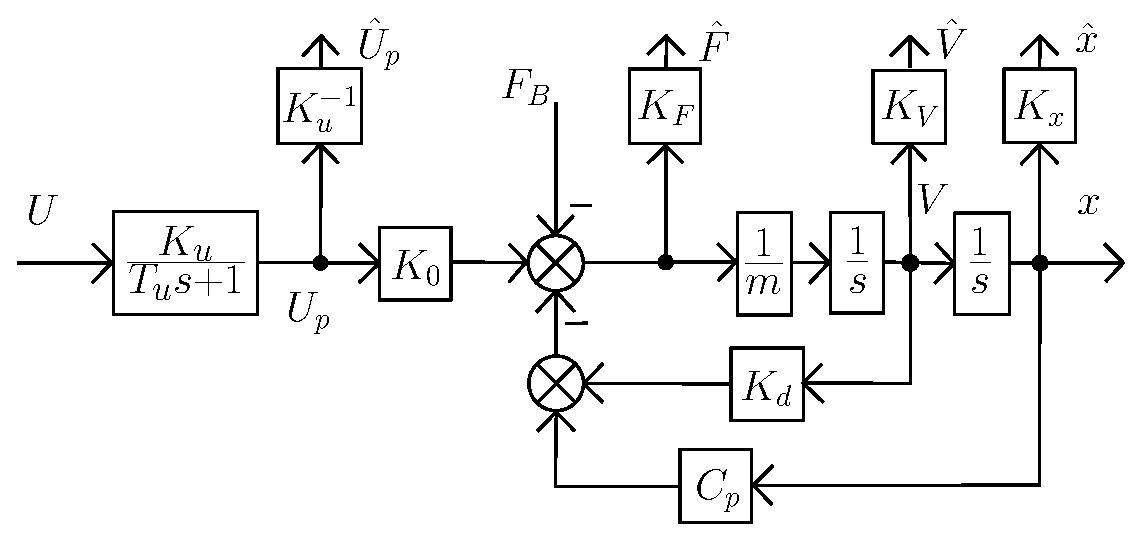
\includegraphics[width = 0.9\textwidth]{Model/structScheme}
		\caption{Структурная схема пьезоэлектрического исполнительного устройства}
		\label{StrScheme}
	\end{figure}
	
	Составим математическую модель в соответствии со структурной схемой, выбрав коэффициенты $K_u^{-1}, K_F, K_V \text{и} K_x$ таки образом, чтобы обеспечить соответствие максимального значения измеряемого сигнала уровню 10 В на выходе измерительного устройства.	Математическая модель, реализованная в среде Simulink, представлена на рисунке \ref{model}.
	\begin{figure}[ht!]
		\centering
		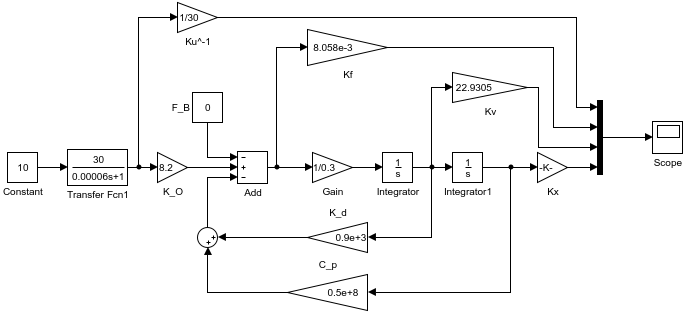
\includegraphics[width = 0.9\textwidth]{Model/mathModel}
		\caption{Схема моделирования пьезоэлектрического исполнительного устройства}
		\label{model}
	\end{figure}
	\newpage
	Результаты математического моделирования приведены на рисунке \ref{baseTP}.
	\begin{figure}[ht!]
		\centering
		\begin{subfigure}[b]{0.49\textwidth}
			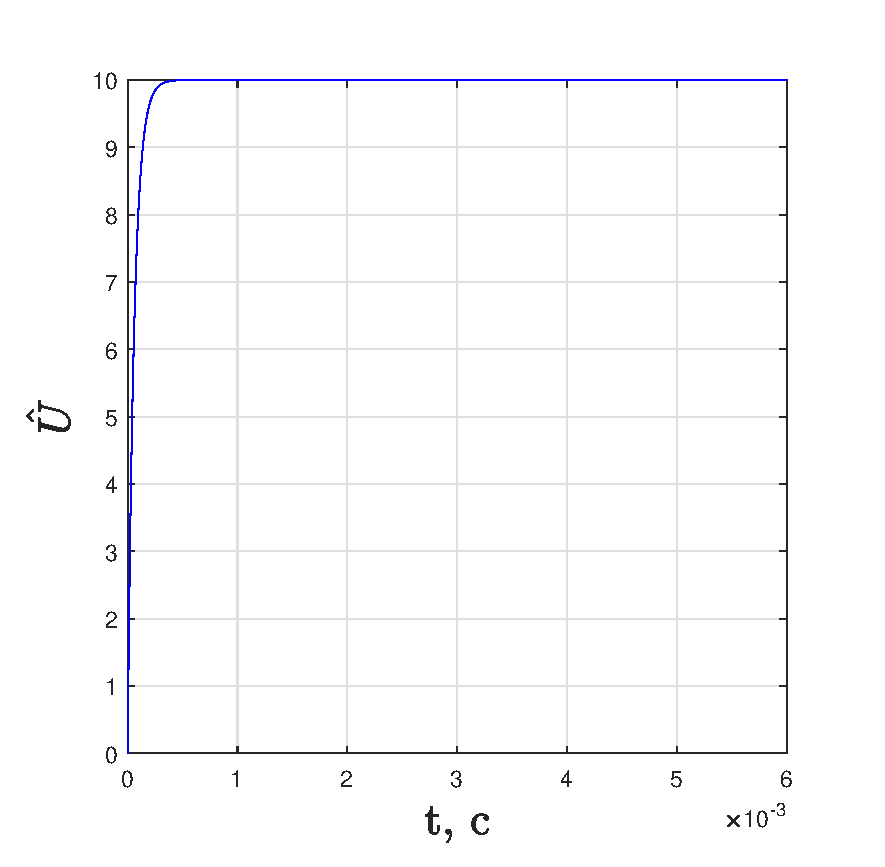
\includegraphics[width = \textwidth]{Base/baseU}
		\end{subfigure}
		\hfill
		\begin{subfigure}[b]{0.49\textwidth}
			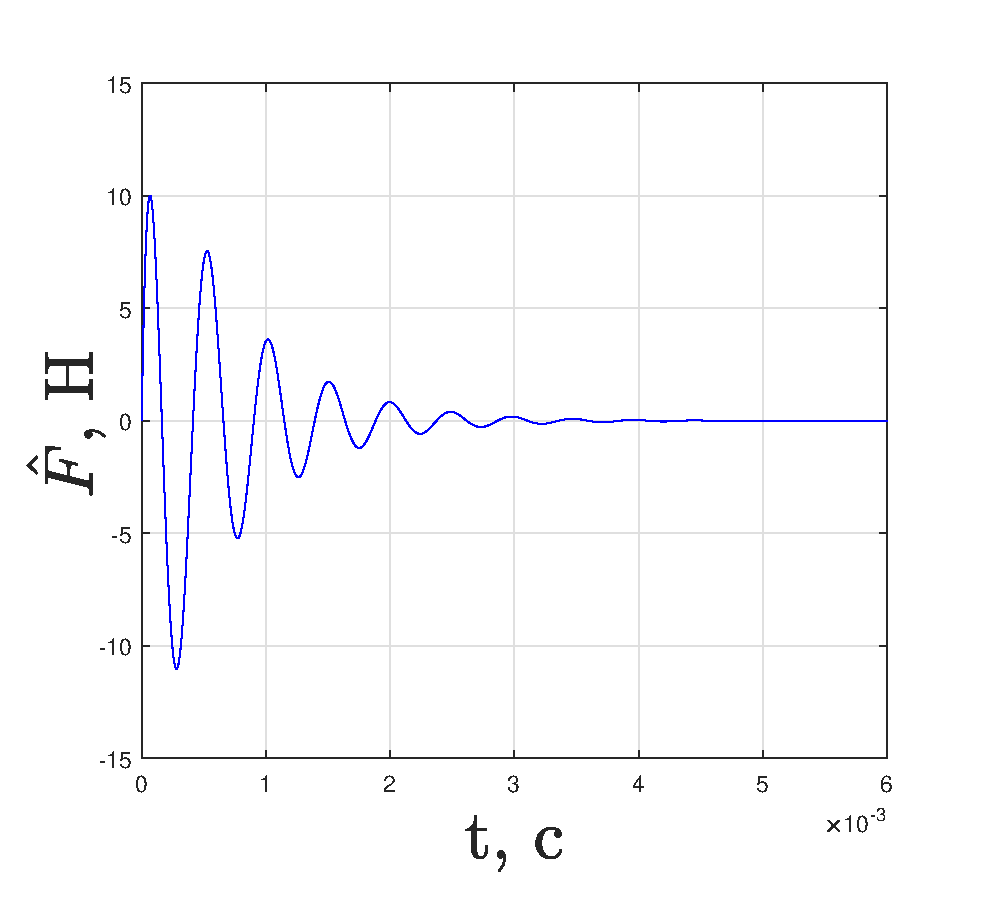
\includegraphics[width = \textwidth]{Base/baseF}
		\end{subfigure}
		
		\begin{subfigure}[b]{0.49\textwidth}
			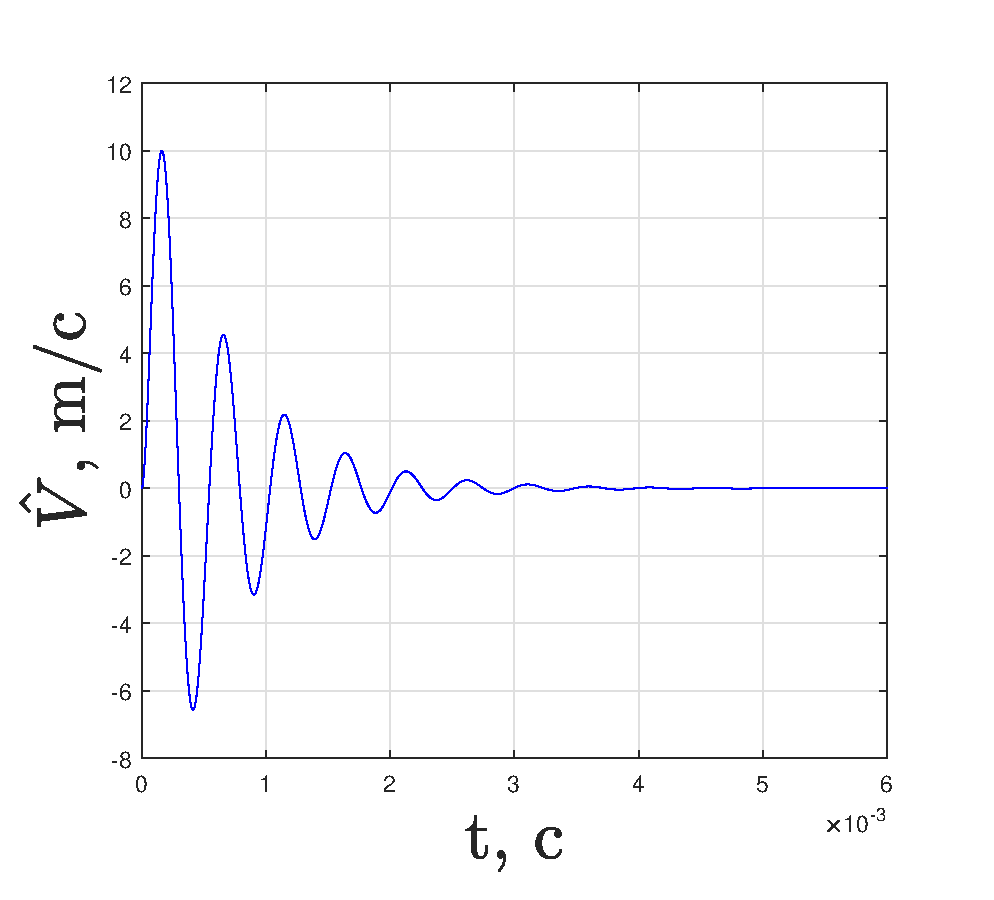
\includegraphics[width = \textwidth]{Base/baseV}
		\end{subfigure}
		\hfill
		\begin{subfigure}[b]{0.49\textwidth}
			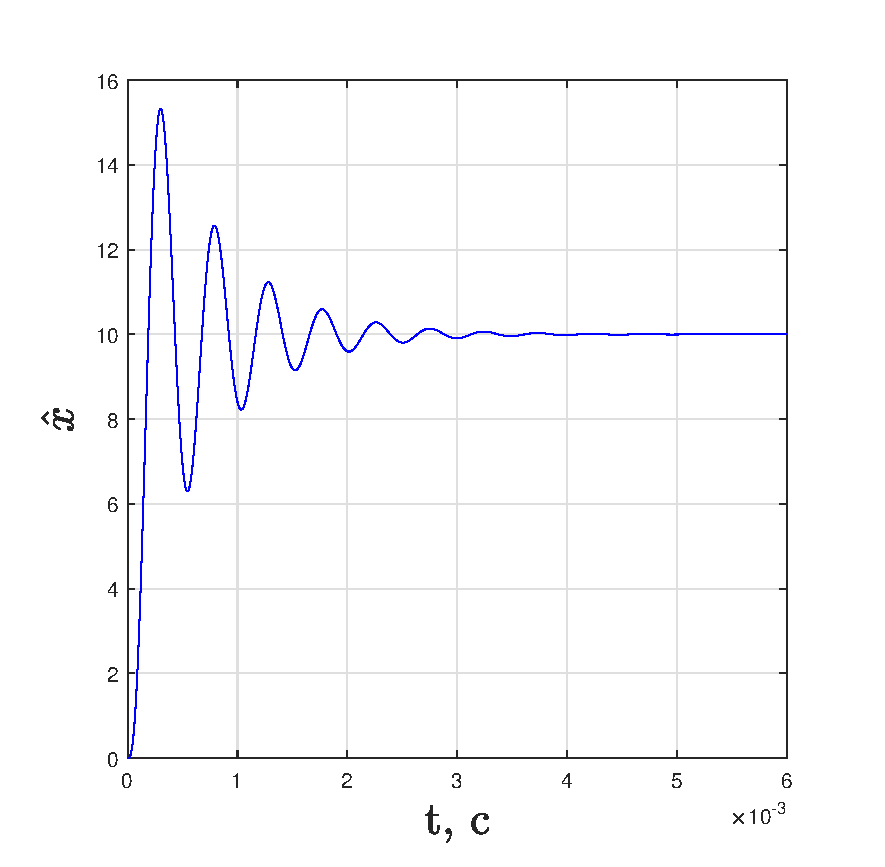
\includegraphics[width = \textwidth]{Base/baseX}
		\end{subfigure}
		\caption{Графики переходных процессов при $U = 10$ и $F_B = 0$}
		\label{baseTP}
	\end{figure}
	\clearpage
	\section{Исследование влияния массы нагрузки на вид переходных процессов}
	\begin{figure}[ht!]
		\centering
		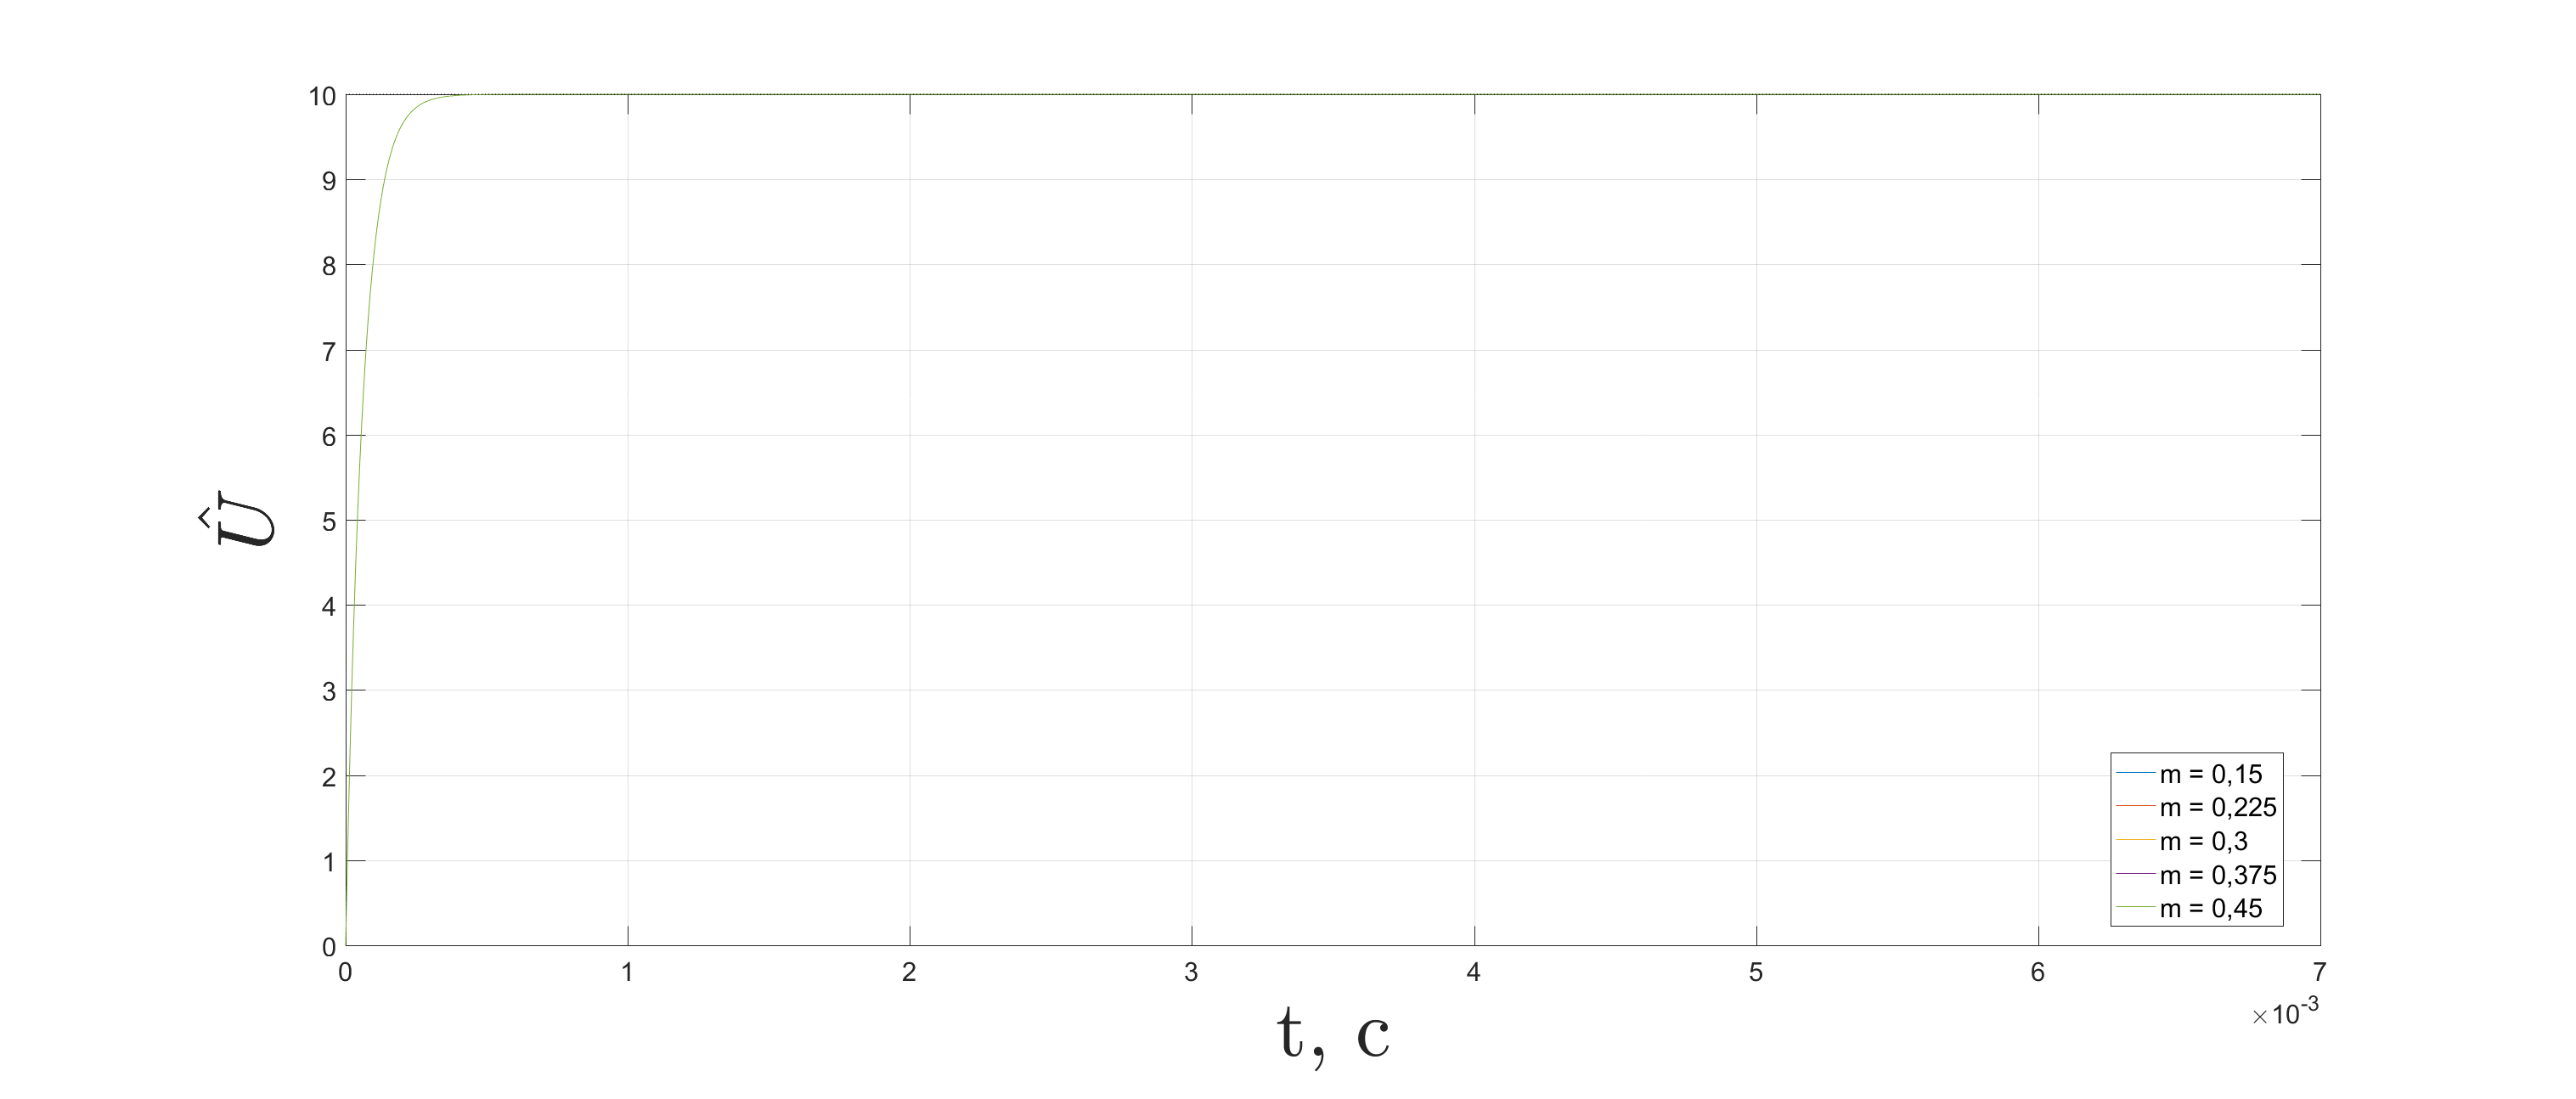
\includegraphics[width = \textwidth]{mvar/mvarU}
		
		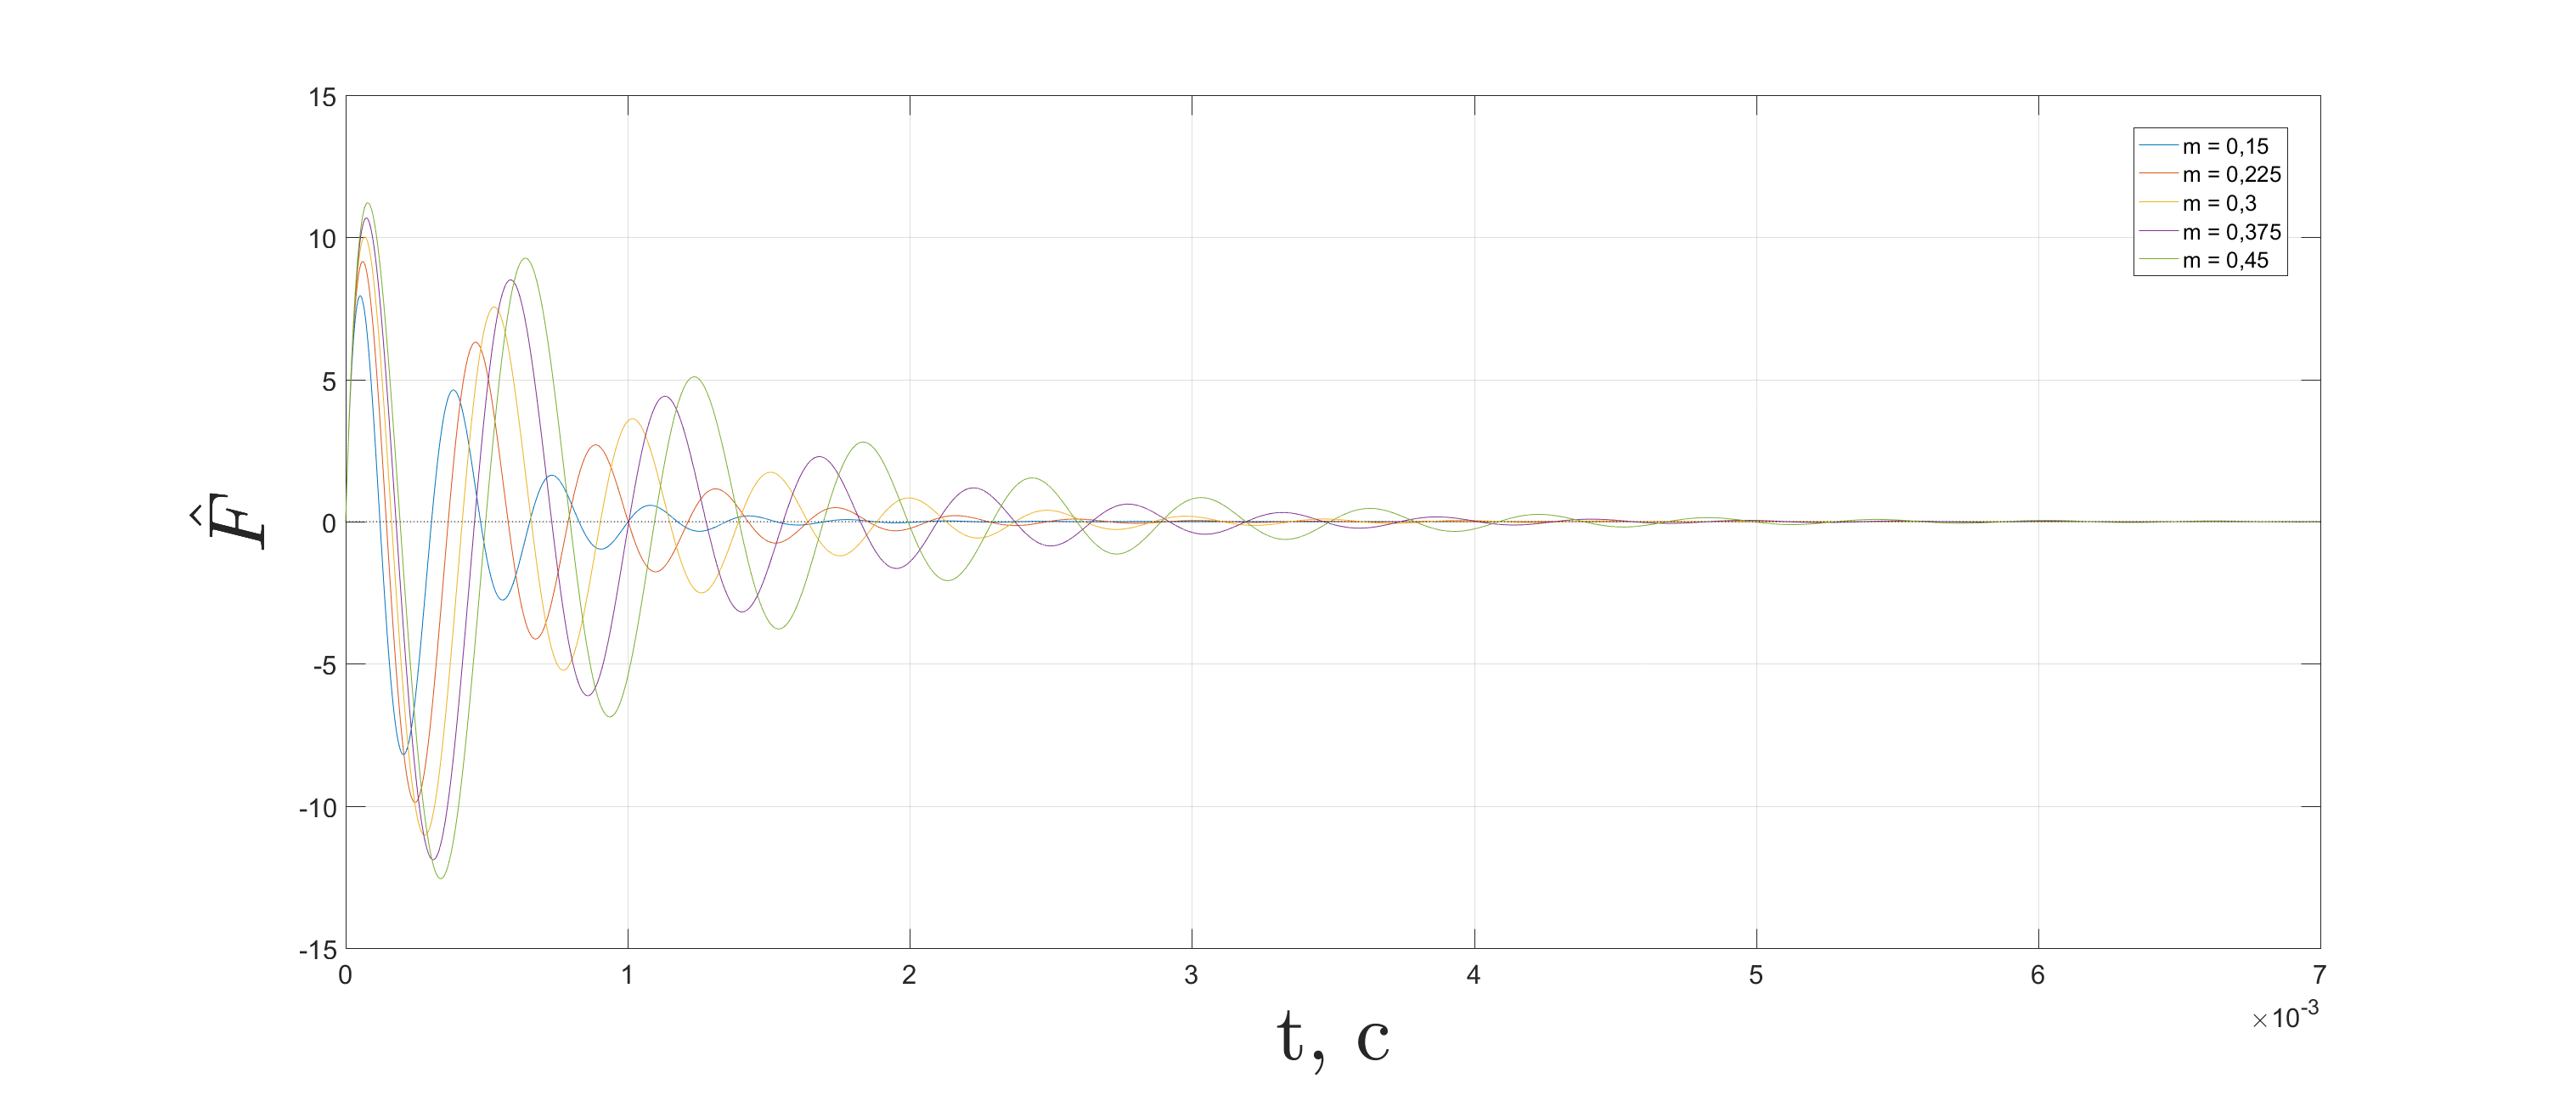
\includegraphics[width = \textwidth]{mvar/mvarF}

		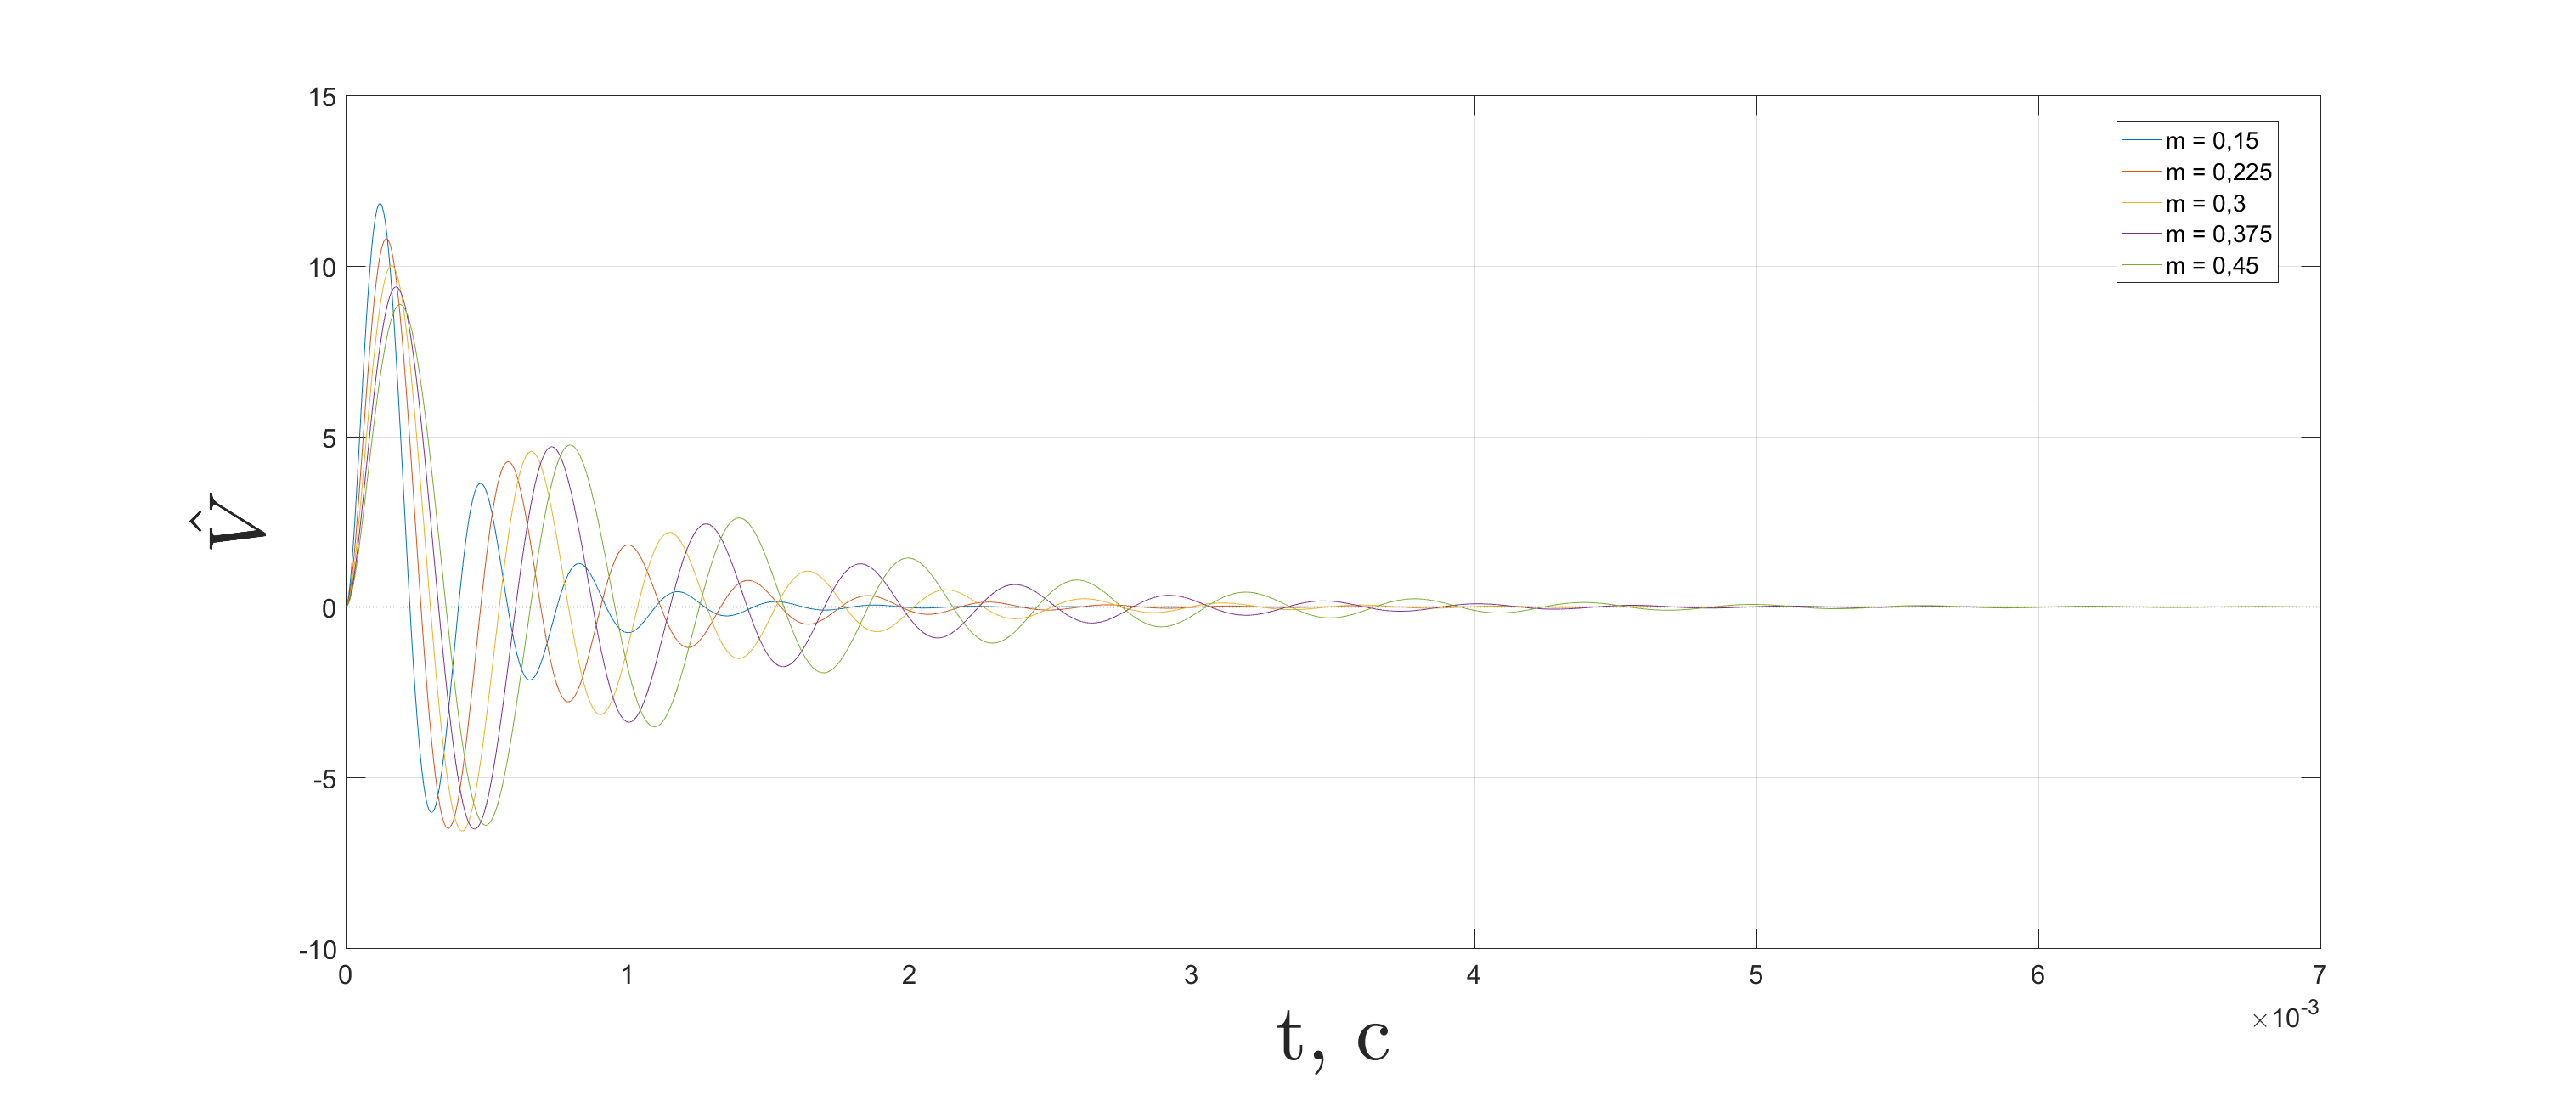
\includegraphics[width = \textwidth]{mvar/mvarV}
	\end{figure}
	\begin{figure}[ht!]		
		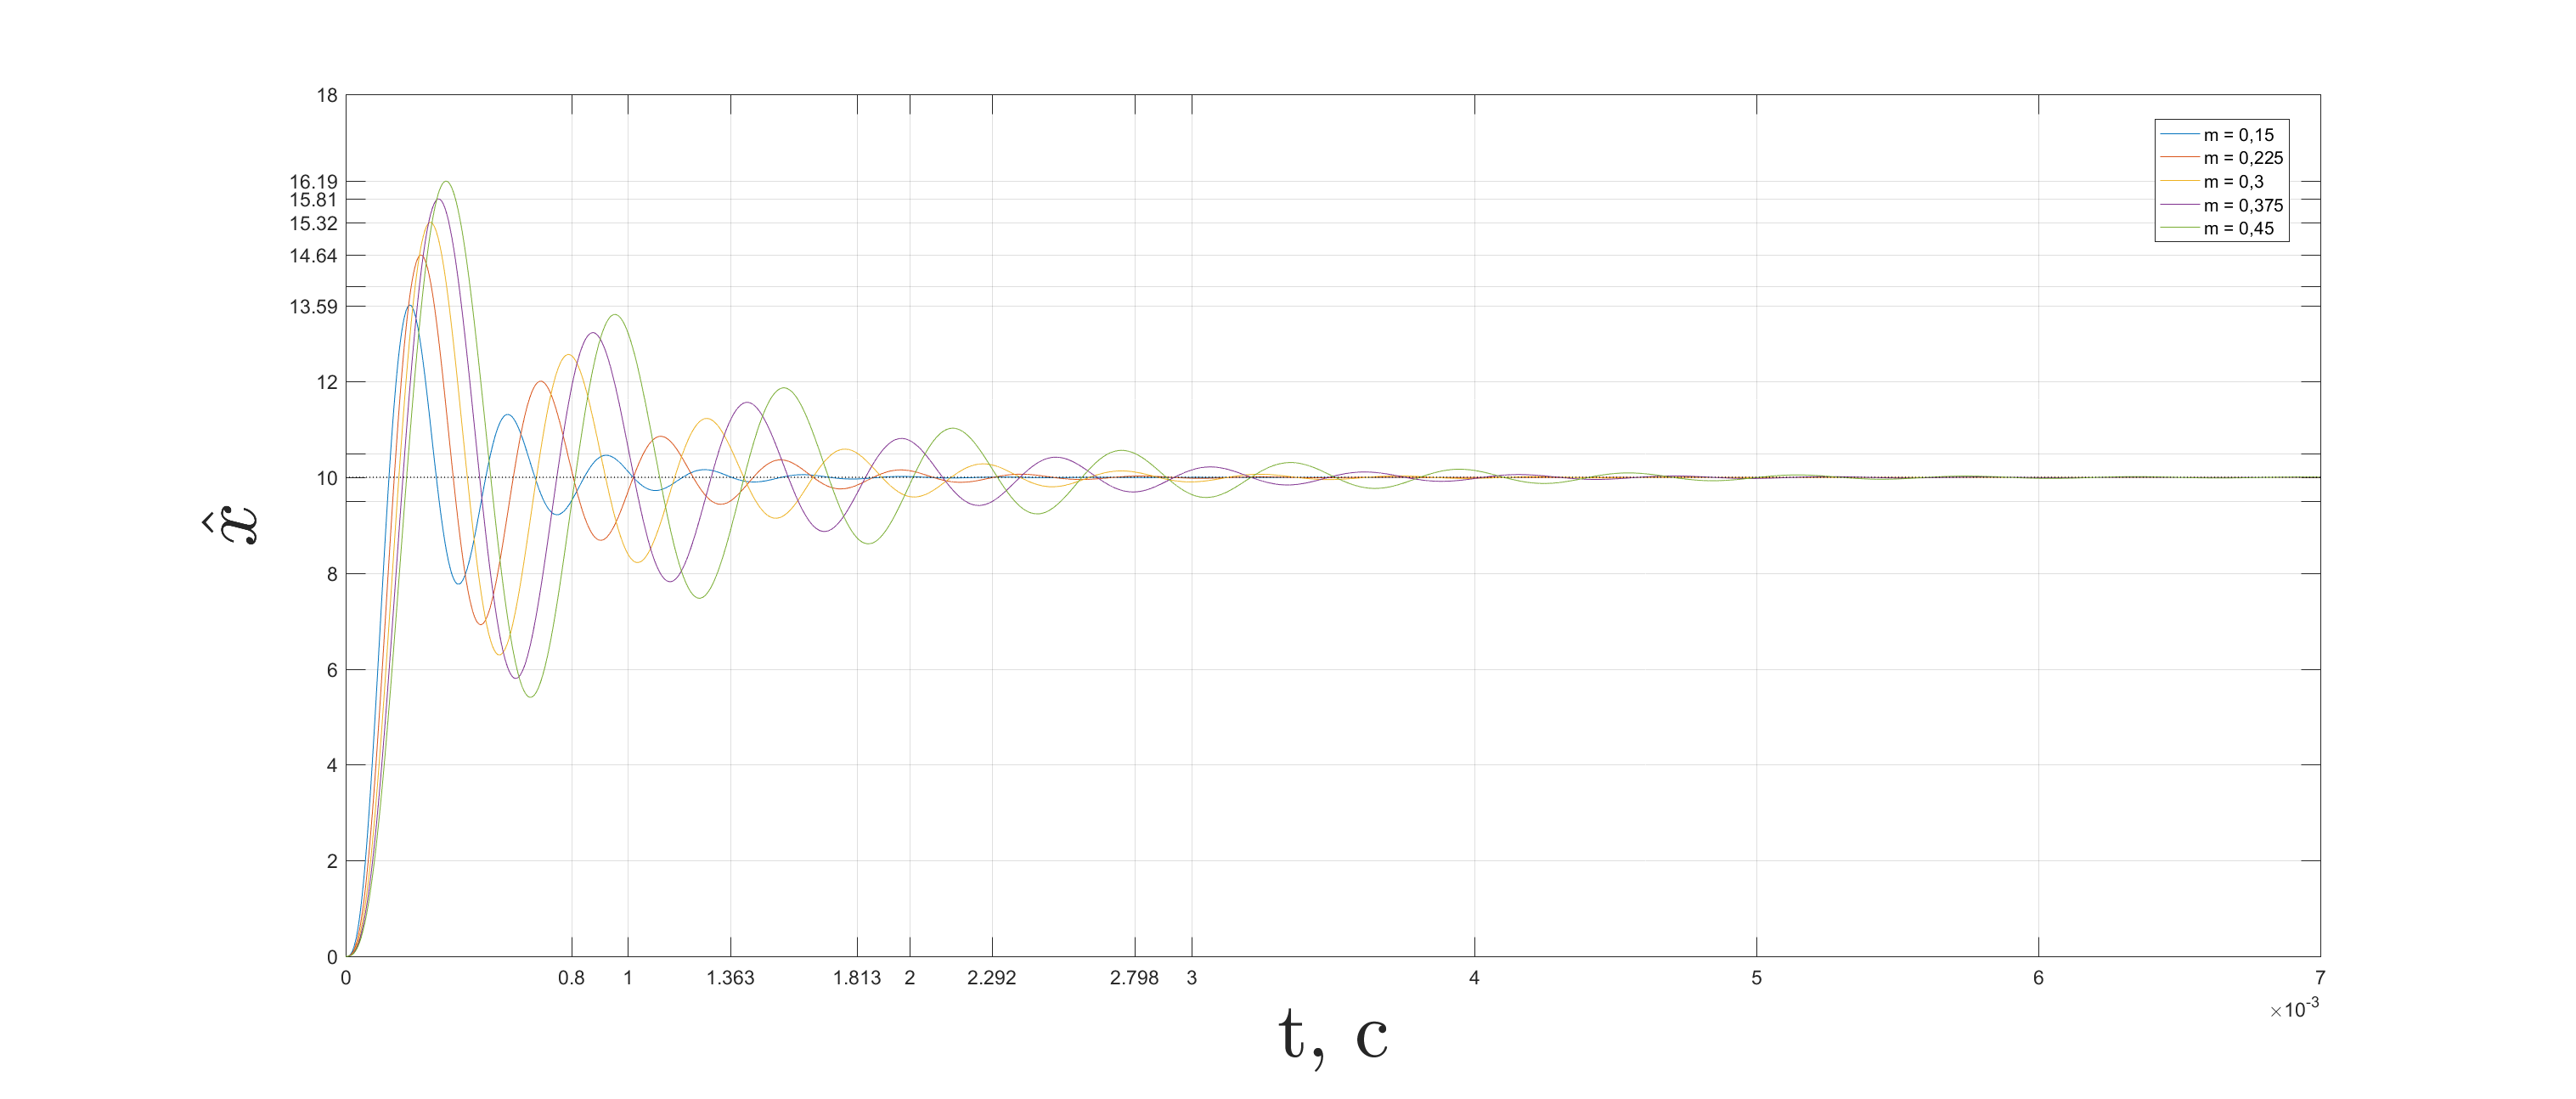
\includegraphics[width = \textwidth]{mvar/mvarX}
		\caption{Графики переходных процессов при различных значениях массы нагрузки}
		\label{mvarGraph}
	\end{figure}
	\newpage
	По результатам моделирования при массе нагрузки $m$, изменяющейся в диапазоне $\pm50\%$, приведённым на рисунке \ref{mvarGraph}, вычислим значения времени переходных процессов, перерегулирования и установившейся величины. Результаты занесём в таблицу \ref{mvarTab}.
	\begin{table}[ht!]
		\caption{Данные переходных процессов при изменяющейся массе нагрузки}
		\begin{tabular}{|c|c|c|c|}
			\hline
			$m,$ кг	& $t_\text{п}, c$	& $\sigma, \%$	& $x_\text{у}$\\
			\hline
			0,15	& 0,8				& 35,9			& 10\\
			\hline
			0,225	& 1,36				& 46,4			& 10\\
			\hline
			0,3		& 1,81				& 53,2			& 10\\
			\hline
			0,375	& 2,29				& 58,1			& 10\\
			\hline
			0,45	& 2,79				& 61,9			& 10\\
			\hline
		\end{tabular}
		\label{mvarTab}
	\end{table}
	
	Можно заметить, что при увеличении массы нагрузки, увеличивается время переходного процесса и значение перерегулирования, в то время как установившееся значение остаётся неизменным.
	\clearpage
	\section{Исследование влияния постоянной времени вольтного усилителя на вид переходных процессов}
	\begin{figure}[ht!]
		\centering
		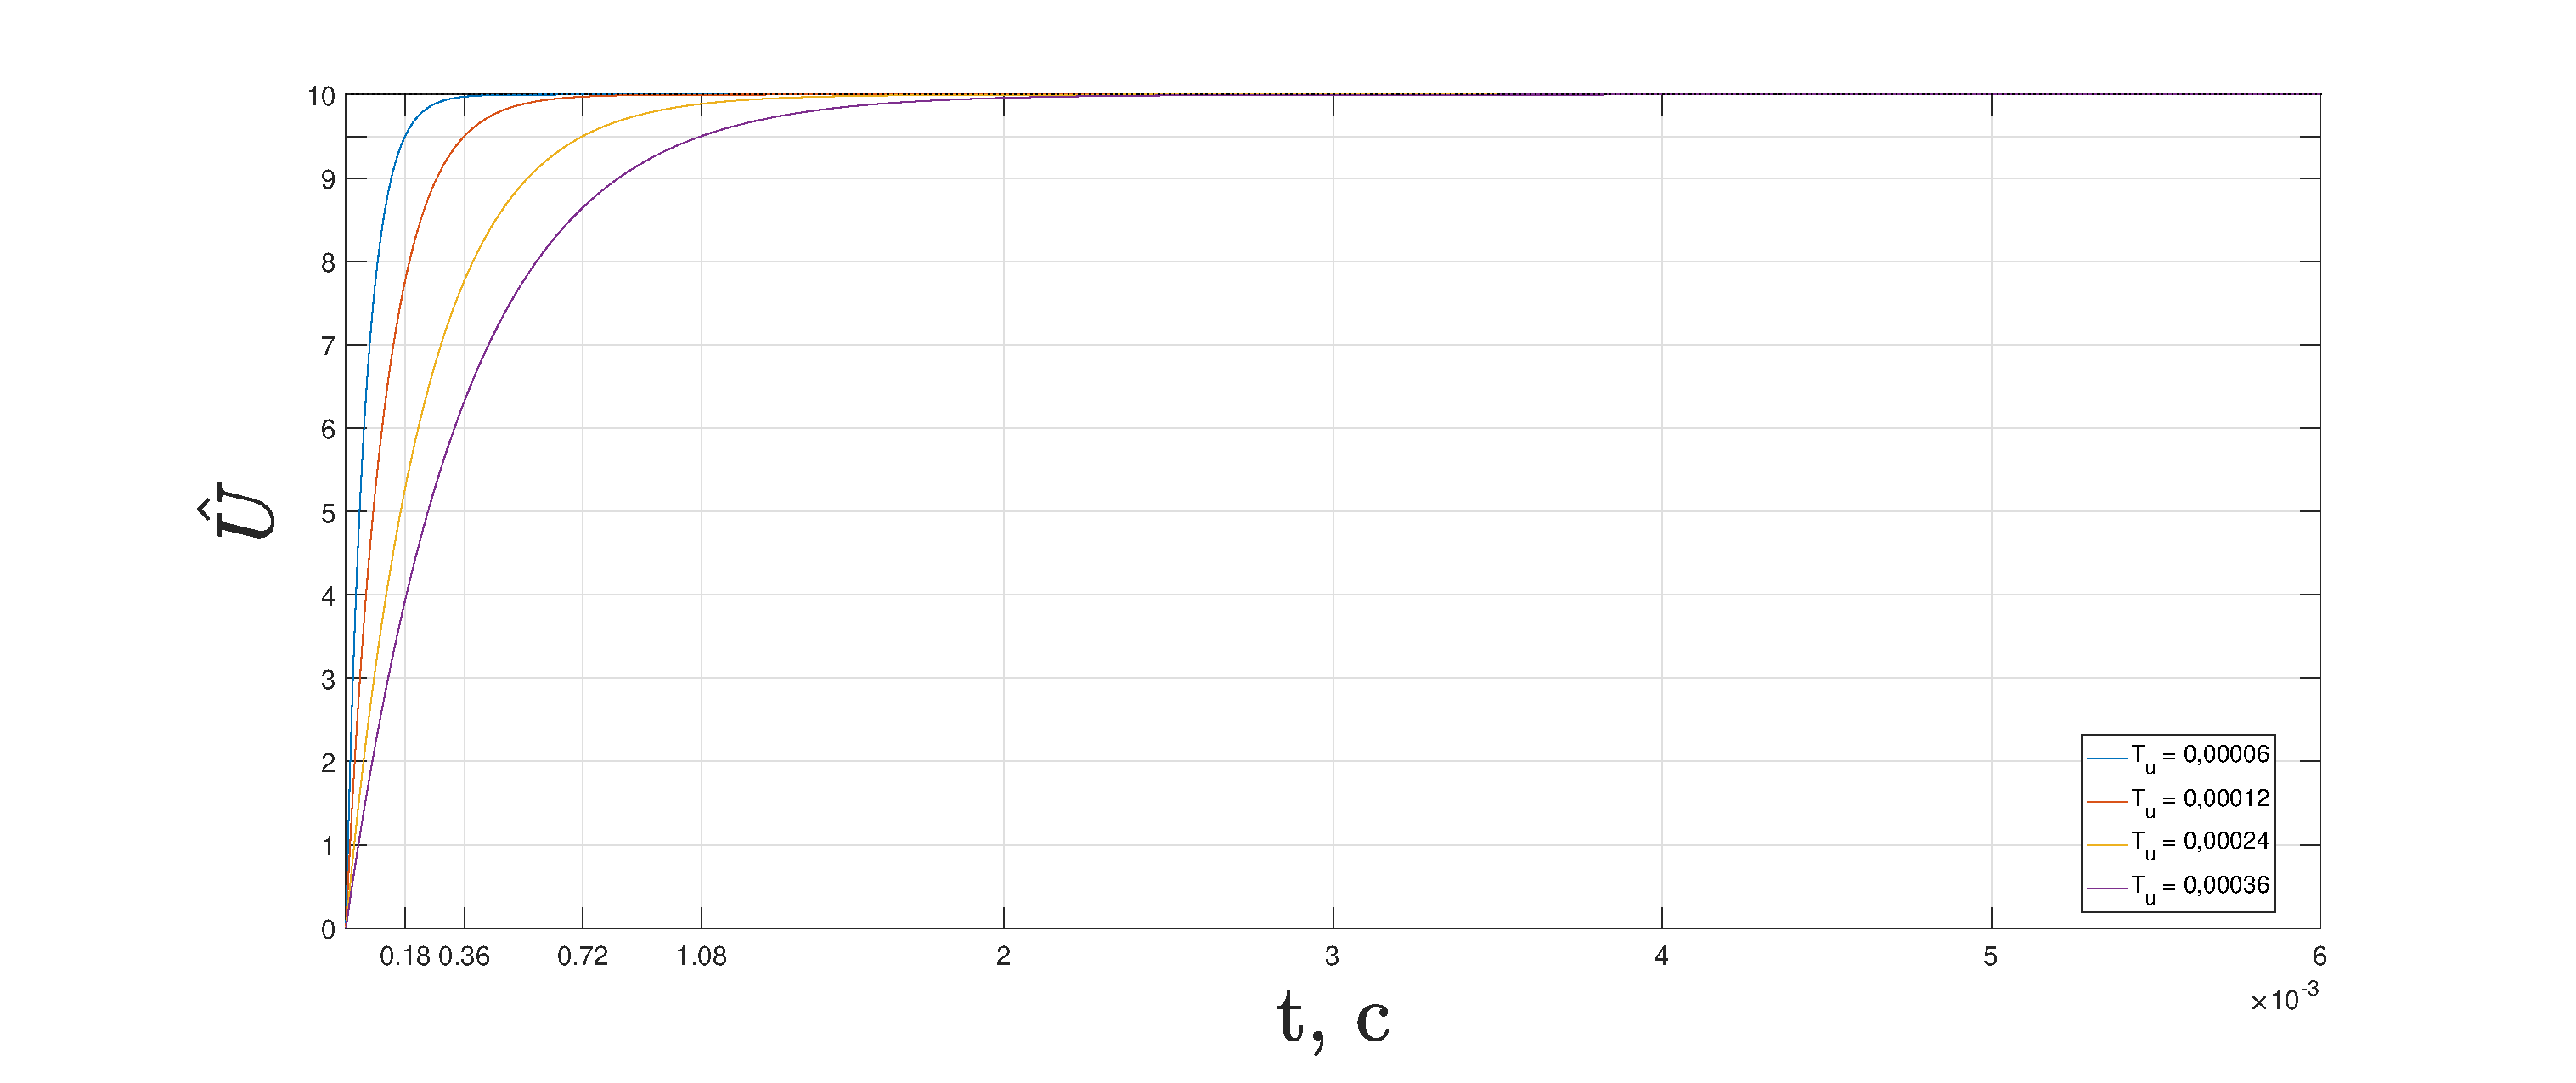
\includegraphics[width = \textwidth]{tvar/tvarU}
		
		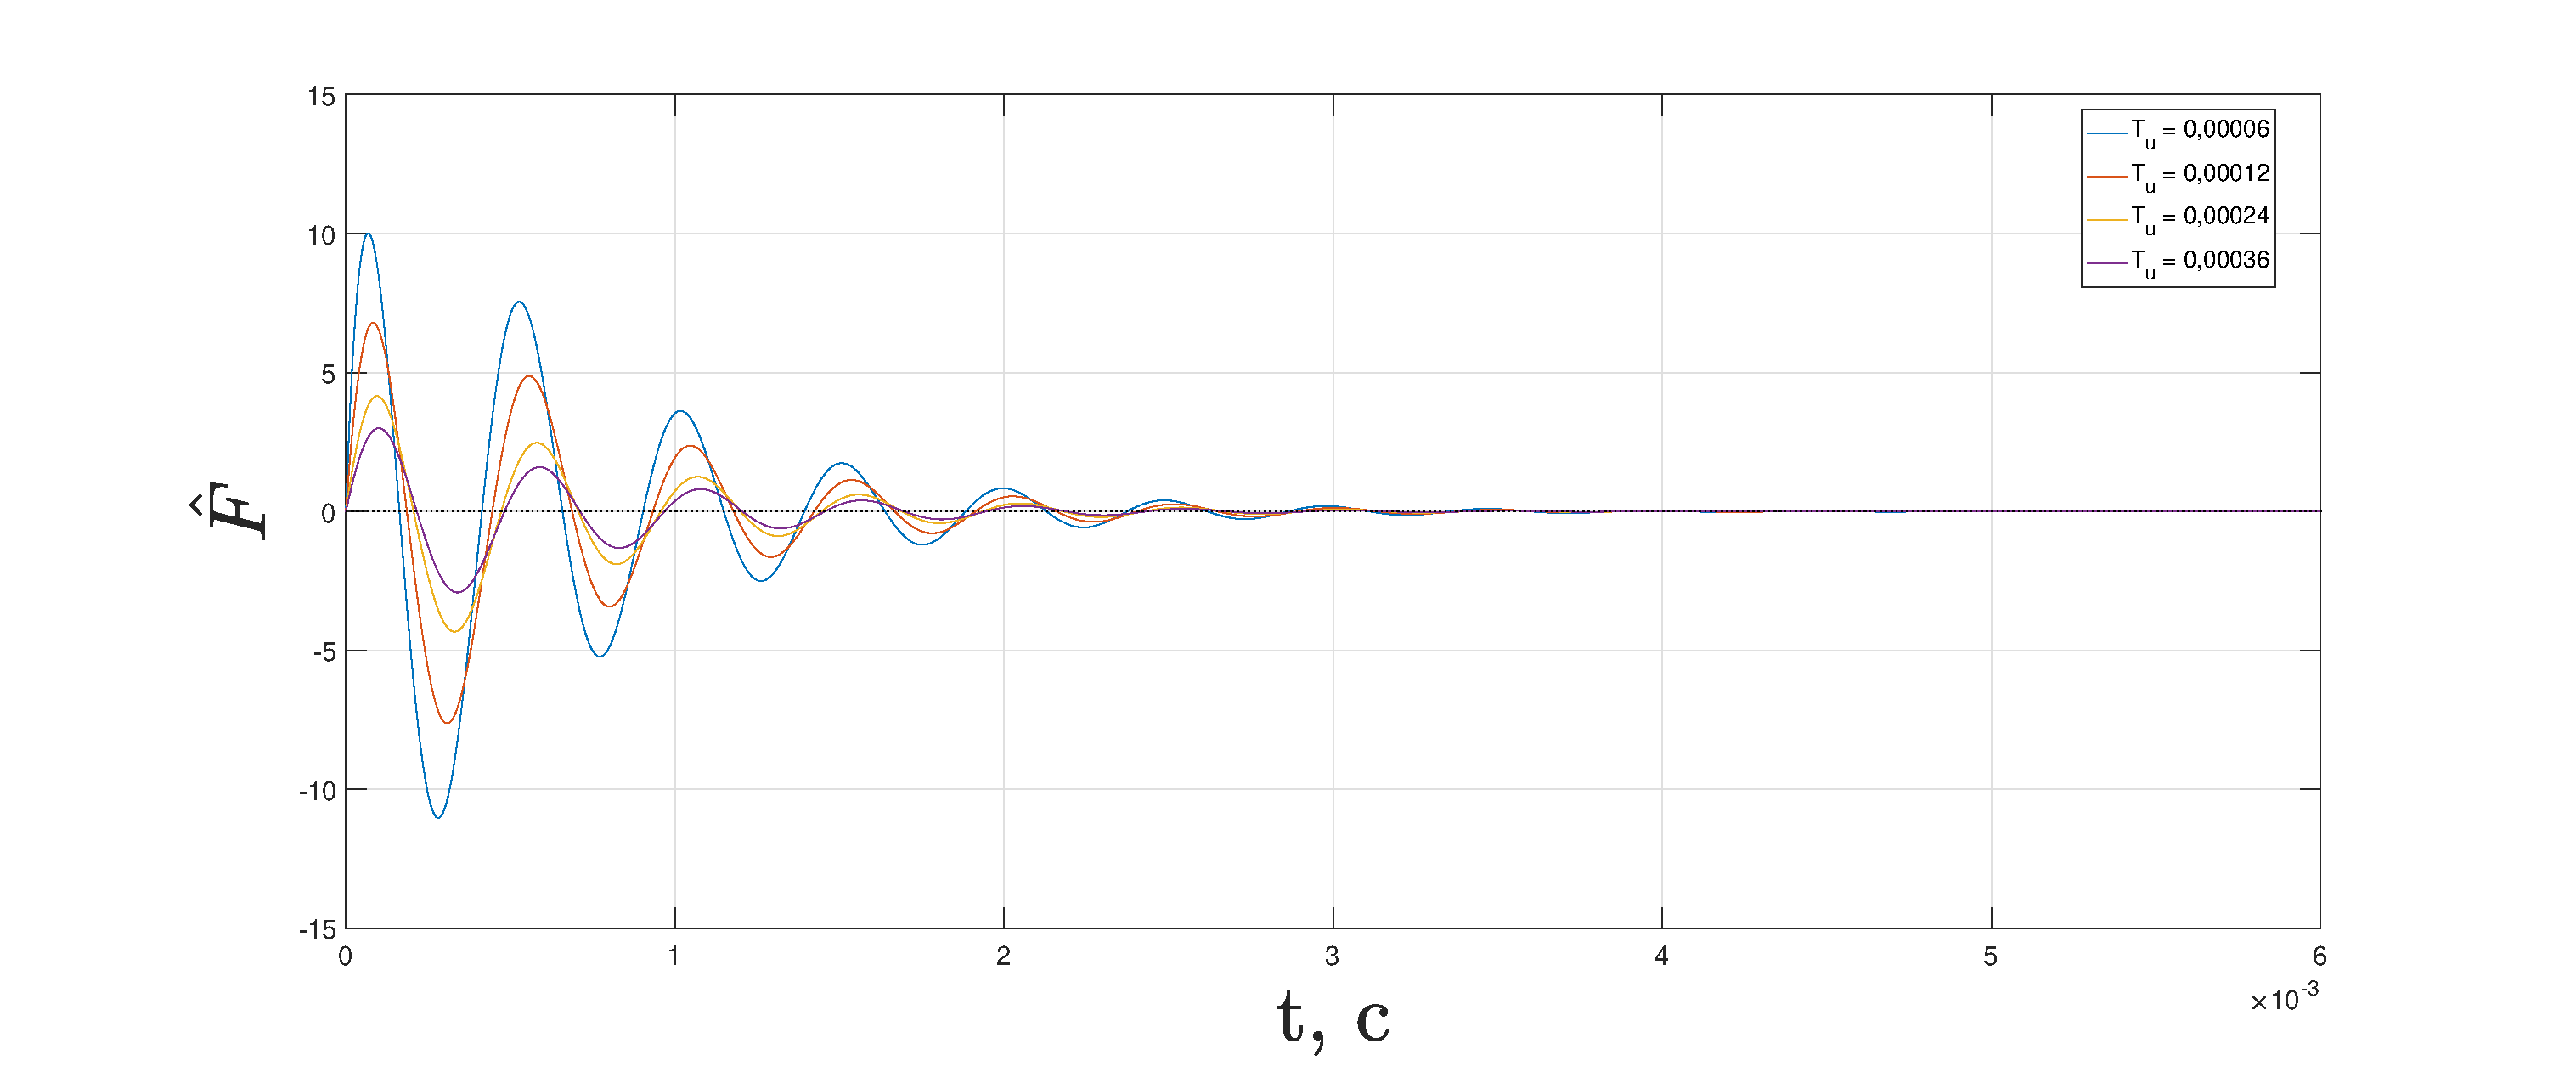
\includegraphics[width = \textwidth]{tvar/tvarF}
		
		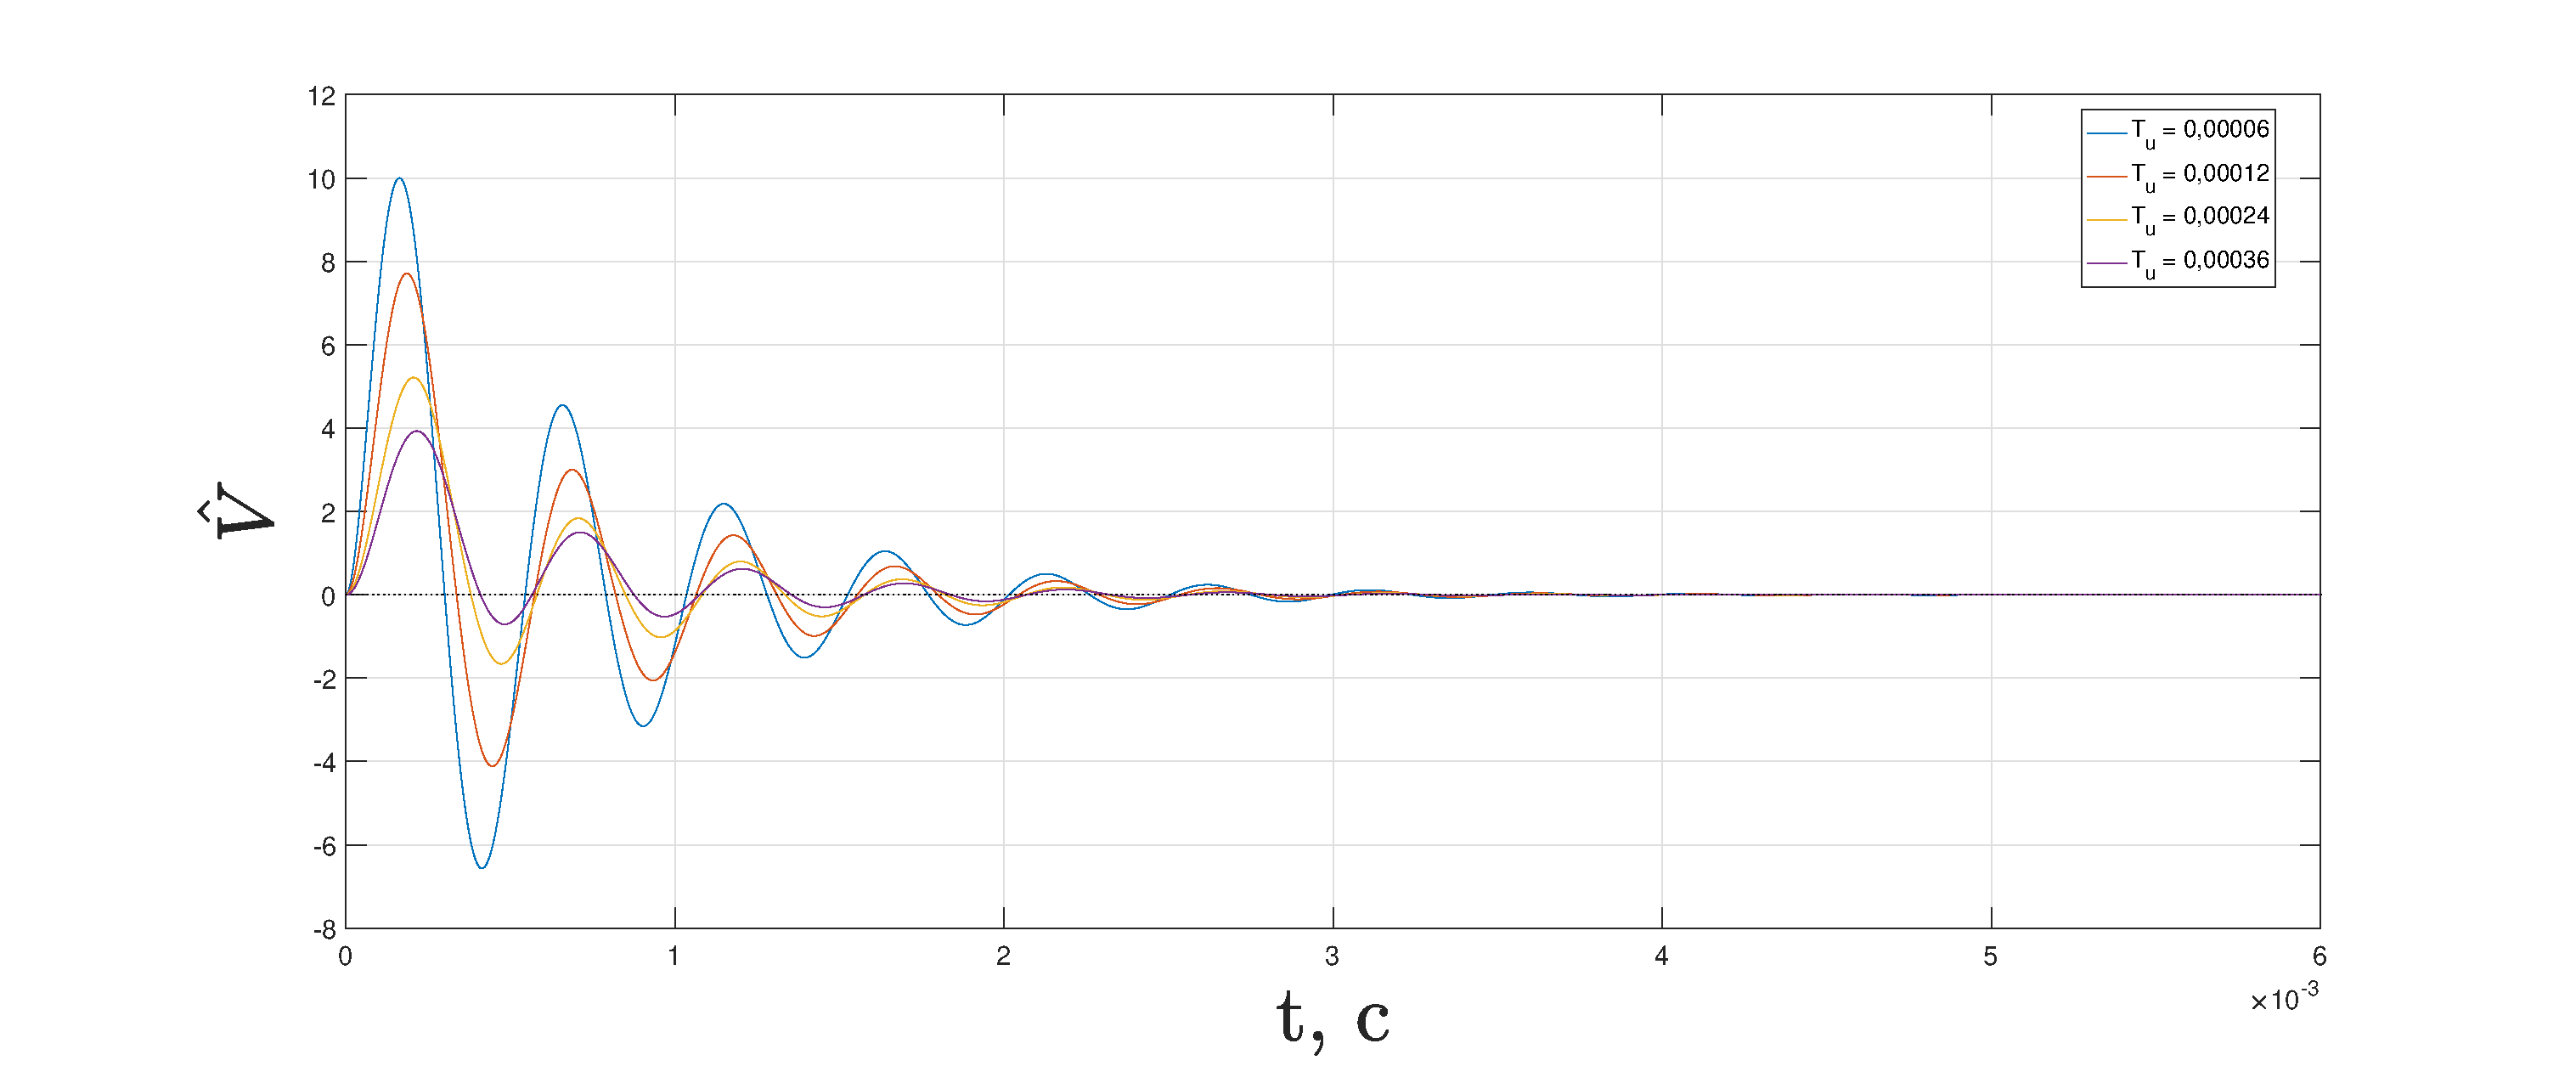
\includegraphics[width = \textwidth]{tvar/tvarV}
	\end{figure}
	\begin{figure}[ht!]
		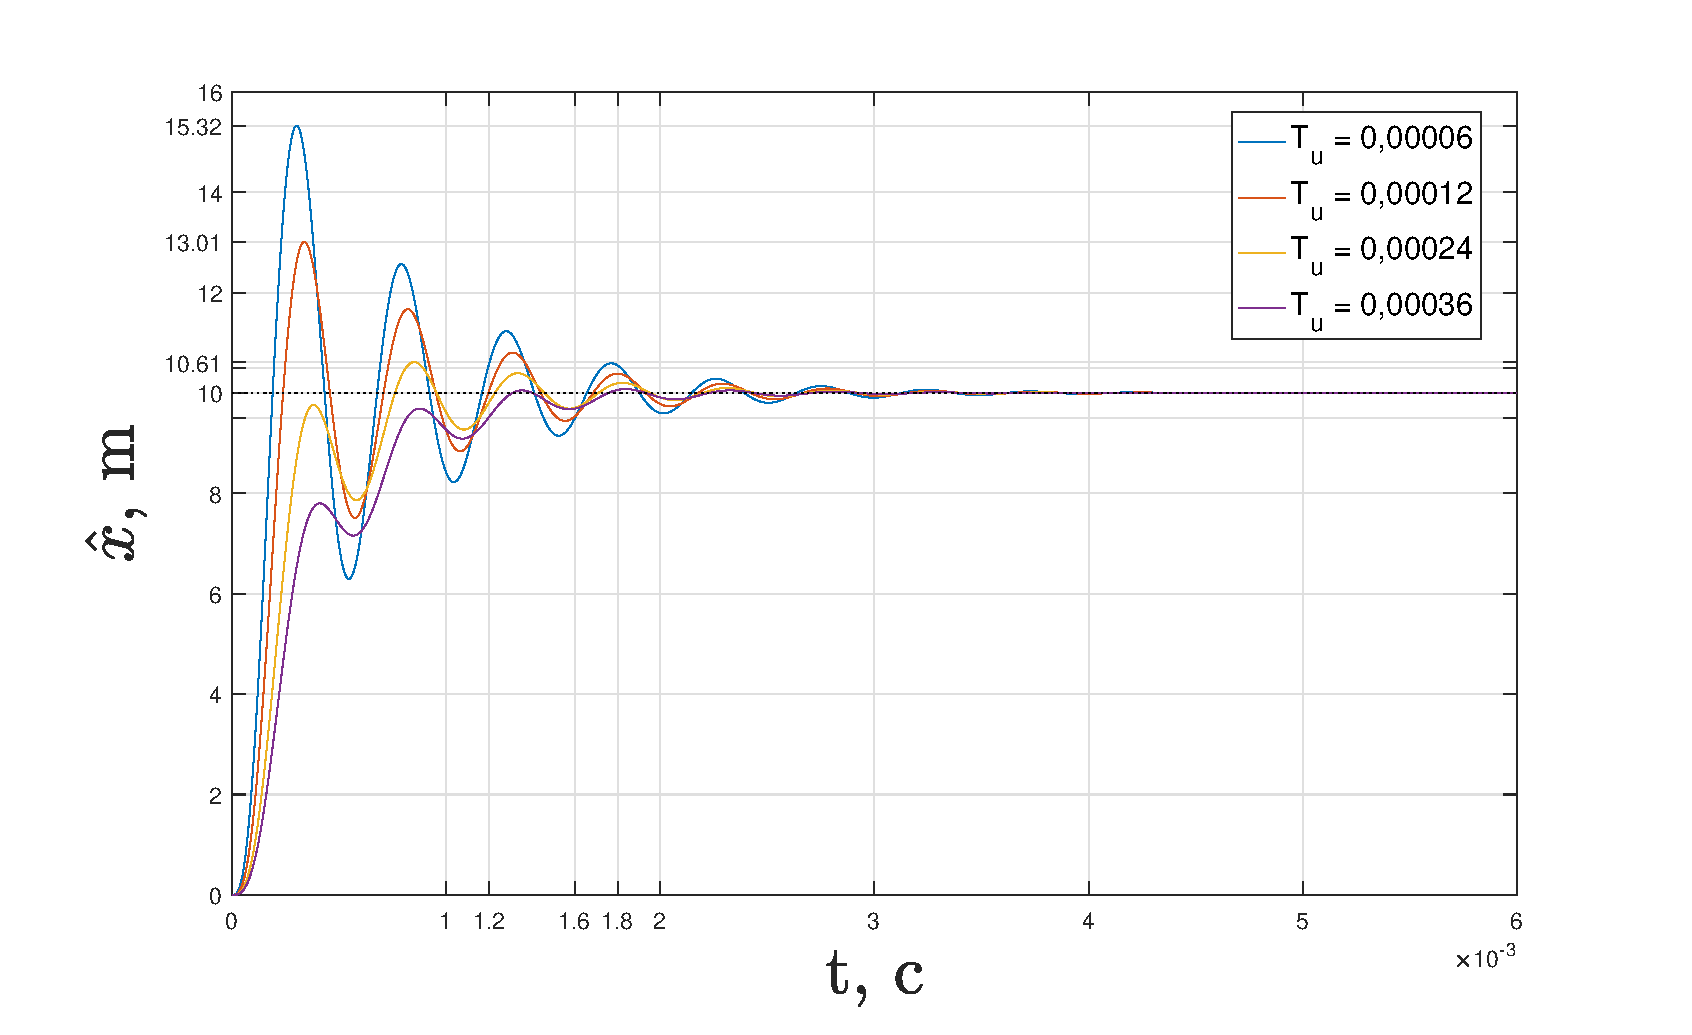
\includegraphics[width = \textwidth]{tvar/tvarX}
		\caption{Графики переходных процессов при различных значениях постоянной времени вольтного усилителя}
		\label{tvarGraph}
	\end{figure}
	\newpage
	По результатам моделирования при постоянной времени $T_u,$ увеличенной в 1, 2, 4 и 6 раз, относительно заданного значения, найдём значения времени переходных процессов, перерегулирования и установившейся величины, а также рассчитаем корни характеристического уравнения передаточной функции. Результаты вычислений занесём в таблицу \ref{tvarTab}.
	\begin{table}[ht!]
		\caption{Данные переходных процессов при изменяющейся постоянной времени вольтного усилителя}
		\begin{tabular}{|c|c|c|c|c|c|c|}
			\hline
			$T_u,$ мс	& $t_\text{п},$ мс	& $\sigma, \%$	& $x_y$	& $s_1$		& $s_2$								& $s_3$								\\\hline
			0,06		& 1,8				& 53,2			& 10	& -16666,67	& \multirow{4}{*}{-1500 + j12822,5}	& \multirow{4}{*}{-1500 - j12822,5} \\\cline{1-5}
			0,12		& 1,6				& 30,1			& 10	& -8333,33	&	& 	\\\cline{1-5}
			0,24		& 1,2				& 6,1			& 10	& -4166,67	& 	&	\\\cline{1-5}
			0,36		& 1,1				& 0,7			& 10	& -2777,78	&	&	\\
			\hline
		\end{tabular}
		\label{tvarTab}
	\end{table}
	
	Из полученных данных следует, что при увеличении постоянной времени вольтного усилителя $T_u$, уменьшаются значения времени переходного процесса, перерегулирования, а установившееся значение остаётся неизменным. Так же с увеличением постоянной времени уменьшается один из корней характеристического уравнения.
	\clearpage
	\section{Исследование влияния коэффициента упругости на вид переходных процессов}
	\begin{figure}[ht!]
		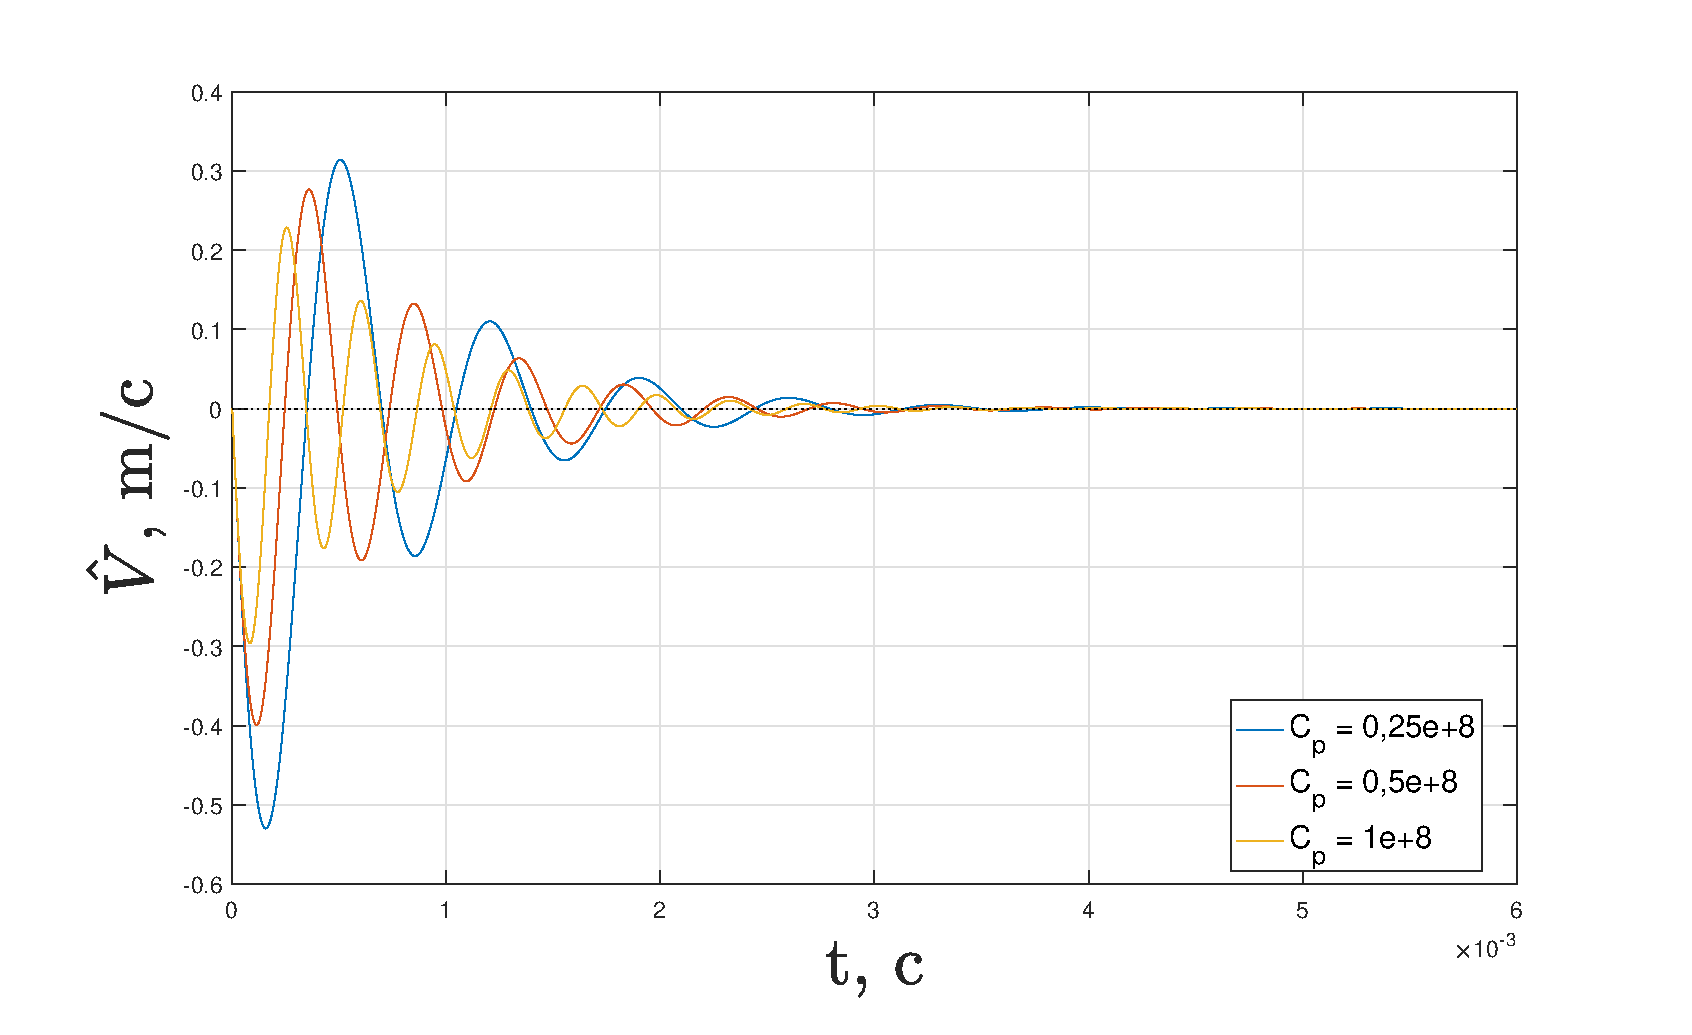
\includegraphics[width = \textwidth]{Cvar/CvarV}
		
		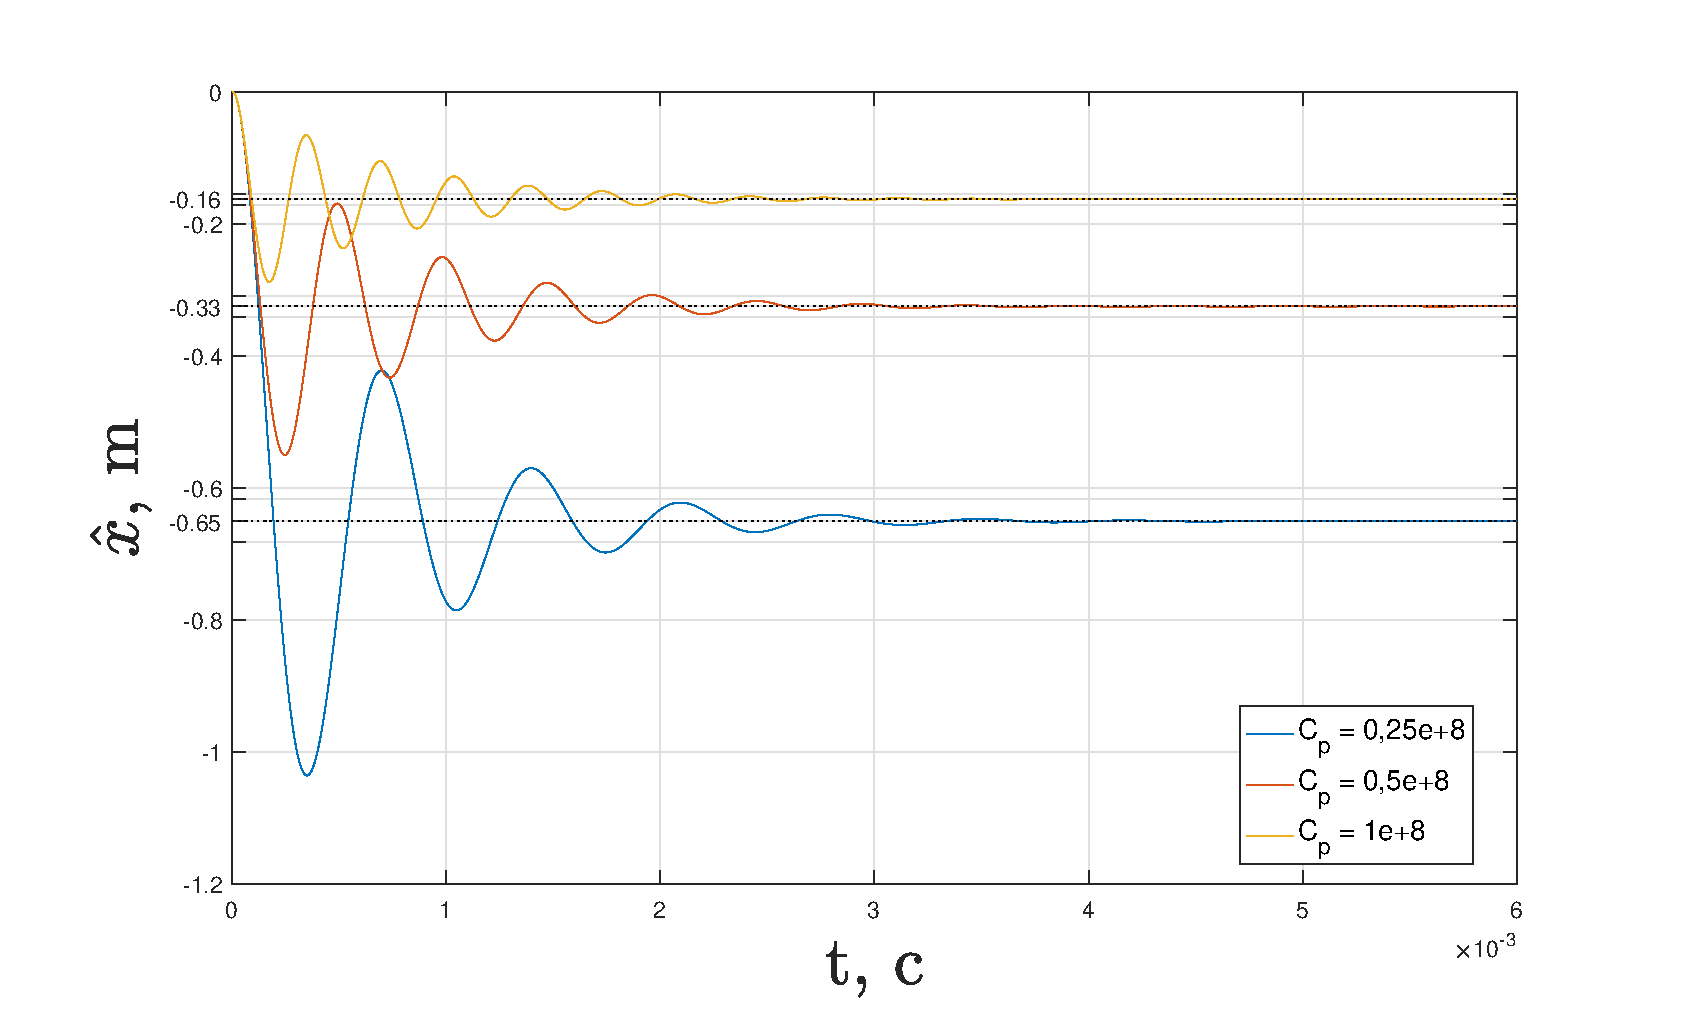
\includegraphics[width = \textwidth]{Cvar/CvarX}
		\caption{Графики переходных процессов при различных значениях коэффициента упругости}
		\label{CvarGraph}
	\end{figure}
	
	По результатам моделирования системы с $U = 0$ и $F_B = 80$ были построены графики переходных процессов по $\hat{V}$ и $\hat{x},$ представленные на рисунке \ref{CvarGraph}. Из графиков видно, что при увеличении коэффициента упругости пьезоэлемента увеличивается смещение установившегося значения $\hat{x}$ относительно 0.
	\clearpage
	\section{Построение АЛАЧХ исполнительного устройства}
	Построим асимптотическую логарифмическую характеристику для нашей системы, описываемой передаточной функцией (\ref{Wpz}). Её не сложно представить в виде колебательного звена:
	\begin{align}
		&&W_\text{кз}(s) = \frac{\displaystyle{\frac{K_0}{C_p}}}{\displaystyle{\frac{m}{C_p}}s^2 + \frac{K_d}{C_p}s + 1}.
	\end{align}
	
	Асимптотическая логарифмическая амплитудная характеристика будет иметь нулевой наклон на уровне 
	\begin{align}
		&&20\log_{10} \displaystyle{\frac{K_0}{C_p}} = 20\log_{10} \displaystyle{\frac{8,2}{0,5\cdot10^8}} = -135,7
	\end{align}
	до сопрягающей частоты 
	\begin{align}
		&&\omega_c = \sqrt{\displaystyle{\frac{C_p}{m}}} = \sqrt{\displaystyle{\frac{0,5\cdot10^8}{0,3}}} = 1,29\cdot10^4 \text{рад/с}.
	\end{align}
	После сопрягающей частоты график пойдёт под наклоном в -40 дБ/дек. Исходя из вышеперечисленных утверждений АЛАЧХ будет выглядит следующим образом:
	\begin{figure}[ht!]
		\centering
		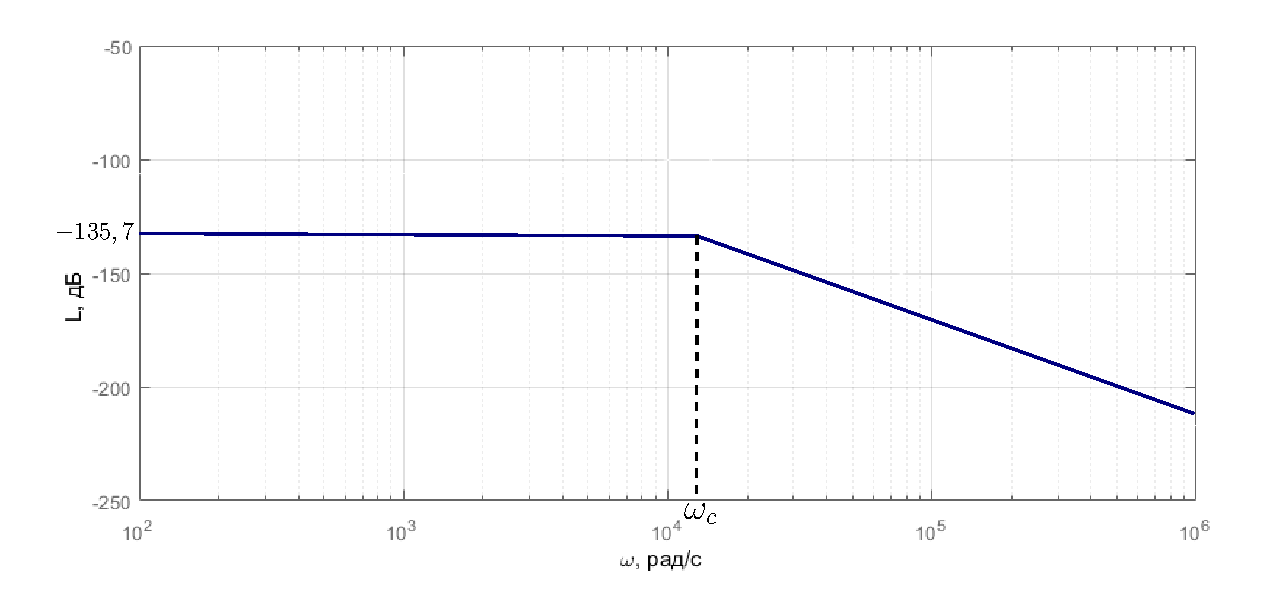
\includegraphics[width = \textwidth]{base/ALAPR}
		\caption{Асимптотическая ЛАЧХ исполнительного устройства}
	\end{figure}
	\clearpage
	\section*{Вывод}
	Исполнительное пьезоэлектрическое устройство можно представить в виде колебательного звена, постоянная времени которого зависит прямо пропорционально от коэффициента упругости и обратно пропорционально от массы нагрузки.
	
	При изменении массы нагрузки изменяются время переходного процесса и значение перерегулирования, оставляя установившееся значение неизменным.
	
	Изменяя постоянную времени вольтного усилителя, мы можем управлять показателями качества переходных процессов пьезоэлектрического устройства. И время переходного процесса, и значение перерегулирования зависят обратно пропорционально от постоянной времени. Установившееся значение на выходе также остаётся неизменным.
	
	При ненулевом внешнем воздействии величина коэффициента упругости пьезоэлемента влияет на установившееся значение. Чем больше значение коэффициента упругости, тем больше на выходе отклонение от 0.
	
\end{document}